\documentclass{article}
\usepackage[utf8]{inputenc}
\usepackage{amsmath}
\usepackage{amssymb}
\usepackage{graphicx}
\usepackage{xcolor}


\begin{document}

\section*{Sparse matrices in CCS format}
We have seen the Compressed Row Storage (CRS) format, we will now look at the very similar Compresses Column Storage format.

\begin{figure}[!hbt]
    \centering
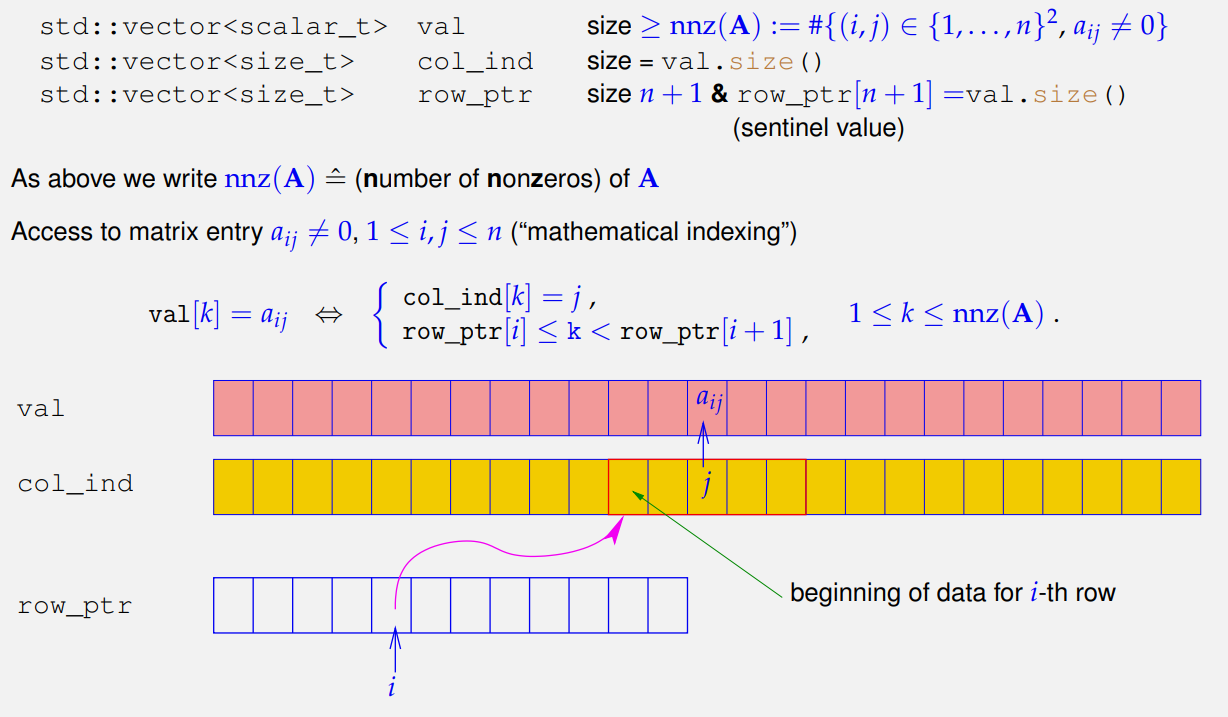
\includegraphics[width=1.0\linewidth]{CRSFormatDef.png}
\end{figure}

\noindent We now have instead of the above arrays \verb|val|, \verb|row_ind| and \verb|col_ptr|. 
\subsection*{2-14.a} 
We are tasked with implementing a \verb|C++| function that given a square matrix $\mathbf{A} \in \mathbb{R}^{n \times n}$ computes the data describing it in CCS format. Let us look at a small example to illustrate what we are supposed to do.
\begin{equation*}
\begin{bmatrix}
    \color{red}1_{1}\color{black} & 0 & 0 & \color{orange}2_{6}\color{black} \\
    0 & 0 & \color{blue}1_{4}\color{black} & 0 \\
    1_{2}\ & 0 & 0 & 3_{7} \\
    0 & \color{green}1_{3}\color{black} & 1_{5} & 2_{\color{teal}8\color{black}}
    \end{bmatrix}
    \begin{matrix}
    \color{red}\verb|col_ptr[0] = 0|\color{black}  \\
    \color{green}\verb|col_ptr[1] = 3|\color{black} \\
\color{blue}\verb|col_ptr[2] = 1|\color{black} \\
\color{orange}\verb|col_ptr[3] = 0|\color{black} \\
\color{teal}\verb|col_ptr[4] = 8|\color{black}
    \end{matrix}  
\end{equation*}
All entries in \verb|col_ptr| we get from the first element in the column, the last entry is the amount of non-zero elements in the matrix and added one to it. The elements in the \verb|val| array are given by
\begin{equation*}
    \begin{matrix}
        0 & 1 & 2 & 3 & 4 & 5 & 6 & 7 \\
        \color{red}1\color{black} & 1 & \color{green}1\color{black} & \color{blue}1\color{black} & 1 & \color{orange}2\color{black} & 3 & 2
    \end{matrix}
\end{equation*}
and the entries of \verb|row_ind| are then given by the corresponding column numbers in the matrix $\mathbf{A}$.
\begin{equation*}
    \begin{matrix}
        0 & 1 & 2 & 3 & 4 & 5 & 6 & 7 \\
        \color{red}0\color{black} & 2 & \color{green}3\color{black} & \color{blue}1\color{black} & 3 & \color{orange}0\color{black} & 2 & 3
    \end{matrix}
\end{equation*}
We can follow the general structure to implement the function. We move through the give matrix column by column, store the row index of the first element in each column and store for each element we encounter the row index and the value in the corresponding array.
\begin{figure}[!hbt]
    \centering
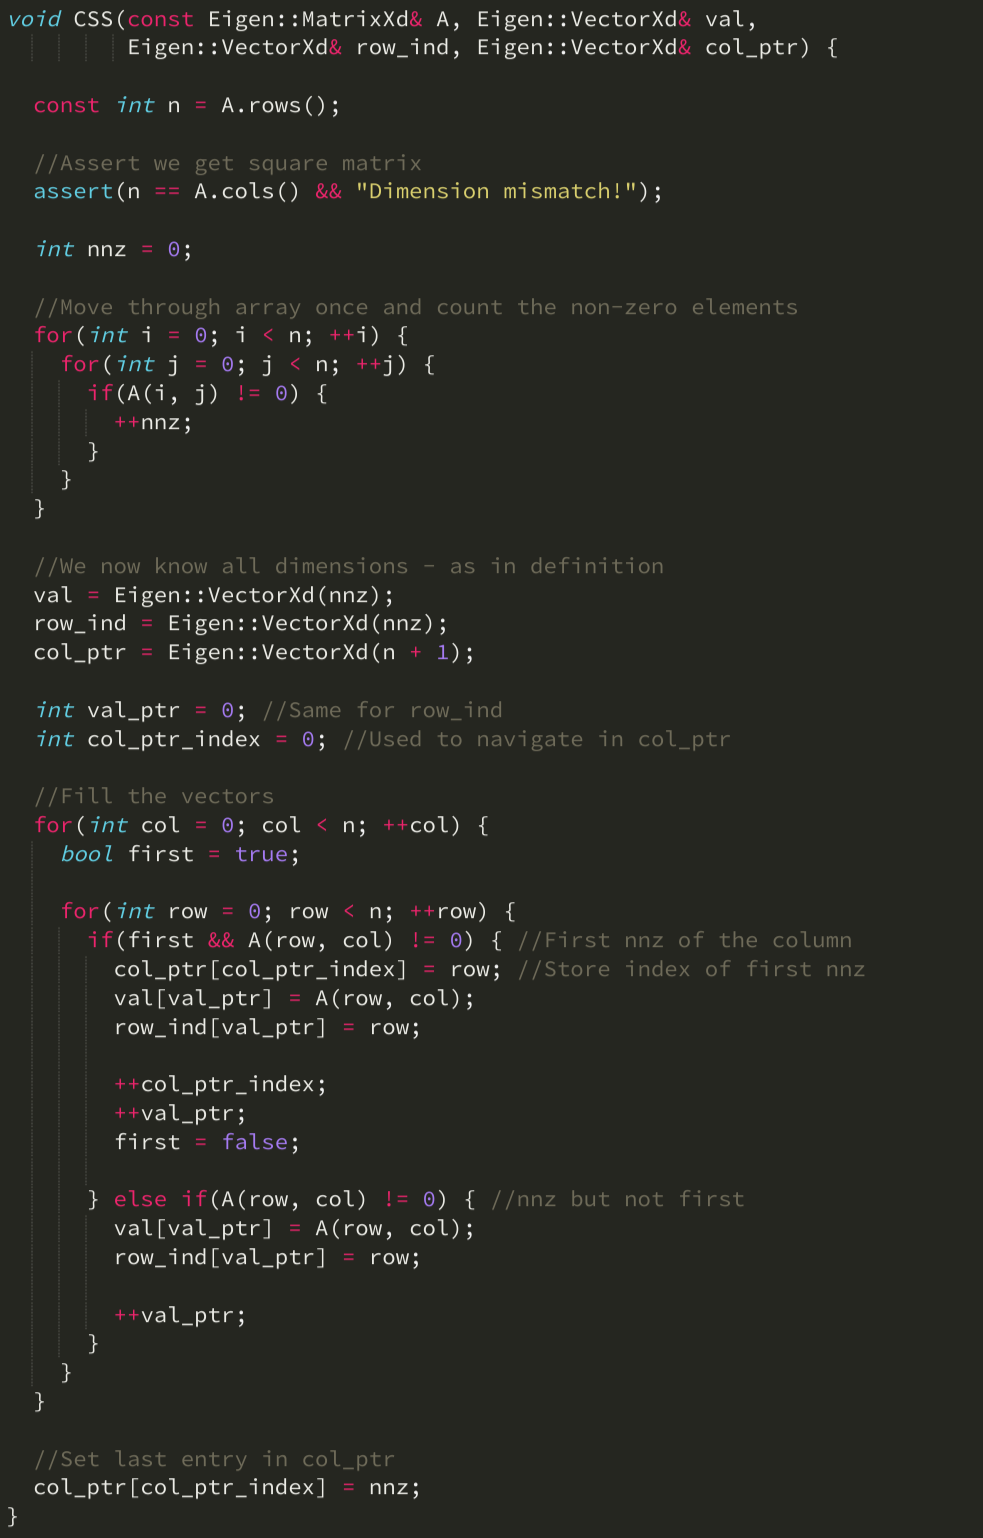
\includegraphics[width=0.9\linewidth]{CCSFormatCode2-14.png}
\end{figure}

\noindent Note that \verb|col_ptr_index| and \verb|col| are the same, they were added to reflect the structure discussed above.
\subsection*{2-14.b}
We are tasked to compute the computational cost of our implementation with respect to the size $n$ of the matrix $\mathbf{A}\in \mathbb{R}^{n \times n}$ and with respect to $\mathrm{nnz}$ the number of non-zero elements in $\mathbf{A}$. We have a computational cost of $\mathcal{O}\left(n^{2}\right)$ as it is dominated by the two double nested for loop which visit every element once and not operations inside of them are made that amount to more than $\mathcal{O}\left(1\right)$ per inner loop iteration. Because we have $\mathrm{nnz} \leq n$ and ideally even $\mathrm{nnz} \ll n$, the asymptotic time complexity does not depend on $\mathrm{nnz}$ and is $\mathcal{O}\left(n^{2}\right)$ regardless of the size of $\mathrm{nnz}$.
\end{document}
